\documentclass[usenames,dvipsnames]{beamer}

\usetheme[bgphoto]{polimi}
% \usetheme{Madrid}
\usepackage[utf8]{inputenc}
\usepackage{appendixnumberbeamer}
\usepackage{array,multirow,booktabs}
\usepackage{lipsum}
\usepackage[font=scriptsize]{caption}
\usepackage{subfig}

% Full instructions available at:
% https://github.com/elauksap/beamerthemepolimi

\title{Gender Discrimination in Data Analysis:\\a Socio-Technical Approach}
\author{Riccardo Corona}
\date{07/10/2021}


\begin{document}
    \begin{frame}
        \maketitle
    \end{frame}
    
    
    \begin{frame}{Table of contents}
      \tableofcontents
    \end{frame}
    
    
    \begin{frame}{Research Context}
        \begin{block}{Data analysis}
            Set of processes for inspecting, cleaning, transforming, and modeling data with the aim of discovering useful information, informing conclusions, and supporting decision making.
        \end{block}
        \begin{block}{Gender discrimination}
            Specific (sub)category of social problems, here expressed in the form of the so-called `\textbf{gender gap}', definable as:
            \begin{quote}
            \emph{A difference between the way men and women are treated in society, or between what men and women do and achieve.}
            \end{quote}
        \end{block}
    \end{frame}
    
    
    \begin{frame}{Scenarios \& Problem Statement}
        \begin{block}{Problem}
            Data and datasets, on which a lot of actions of our daily routine are based, can be \textbf {unfair}. Unfair, or better to say, \textbf{biased} data, may influence, directly or indirectly, our perception of reality, and lead us to make decisions that, although seemingly fair and just, contain in turn bias, and discriminate against individuals or groups of individuals.
        \end{block}
        \begin{exampleblock}{Example scenarios}
            \begin{itemize}
                \item \textcolor{greenPolimi}{COMPAS} tool used in the U.S. to predict recidivism risk biased against Black people (2016).
                \item \textcolor{greenPolimi}{Amazon} software to screen candidates for employment biased against women (2015).
            \end{itemize}
        \end{exampleblock}
    \end{frame}
    
    
    \begin{frame}{Sociological Perspective -- Data \& Statistics}
        \begin{figure}
            \subfloat{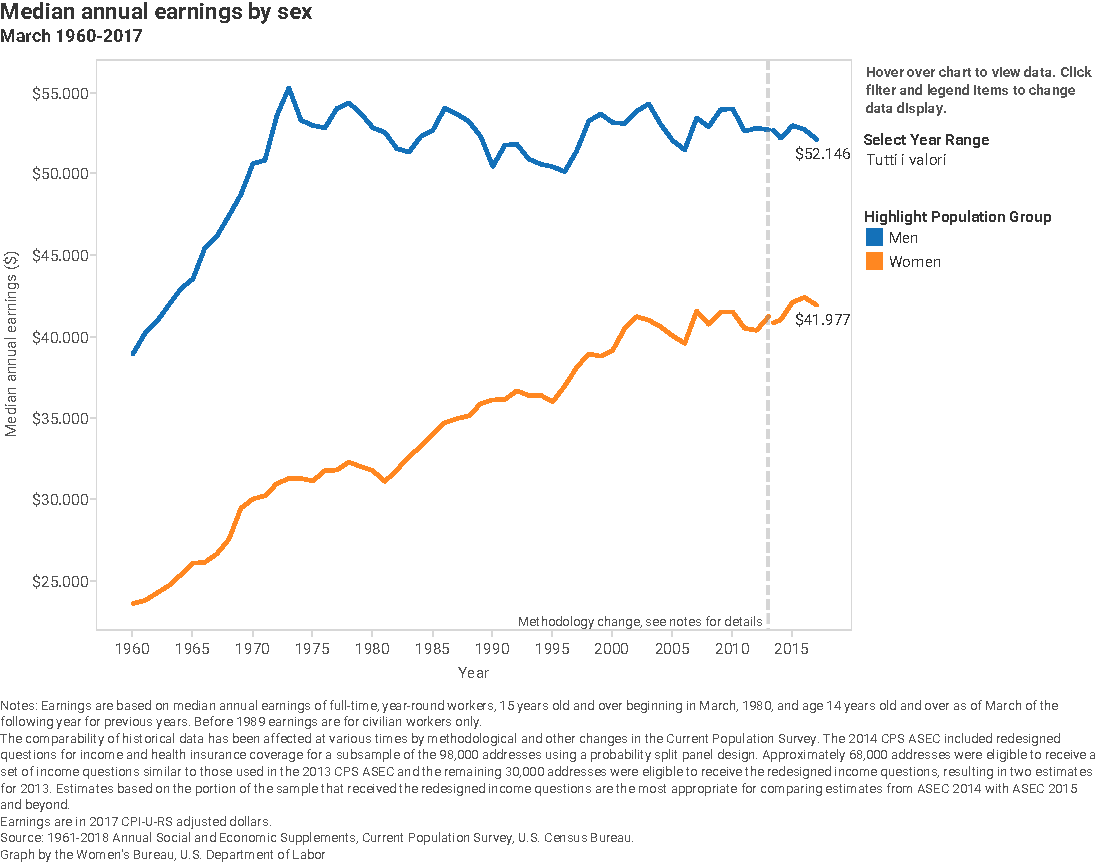
\includegraphics[width=0.475\textwidth]{figures/dol_earnings_by_sex.pdf}}
            \hfill
            \subfloat{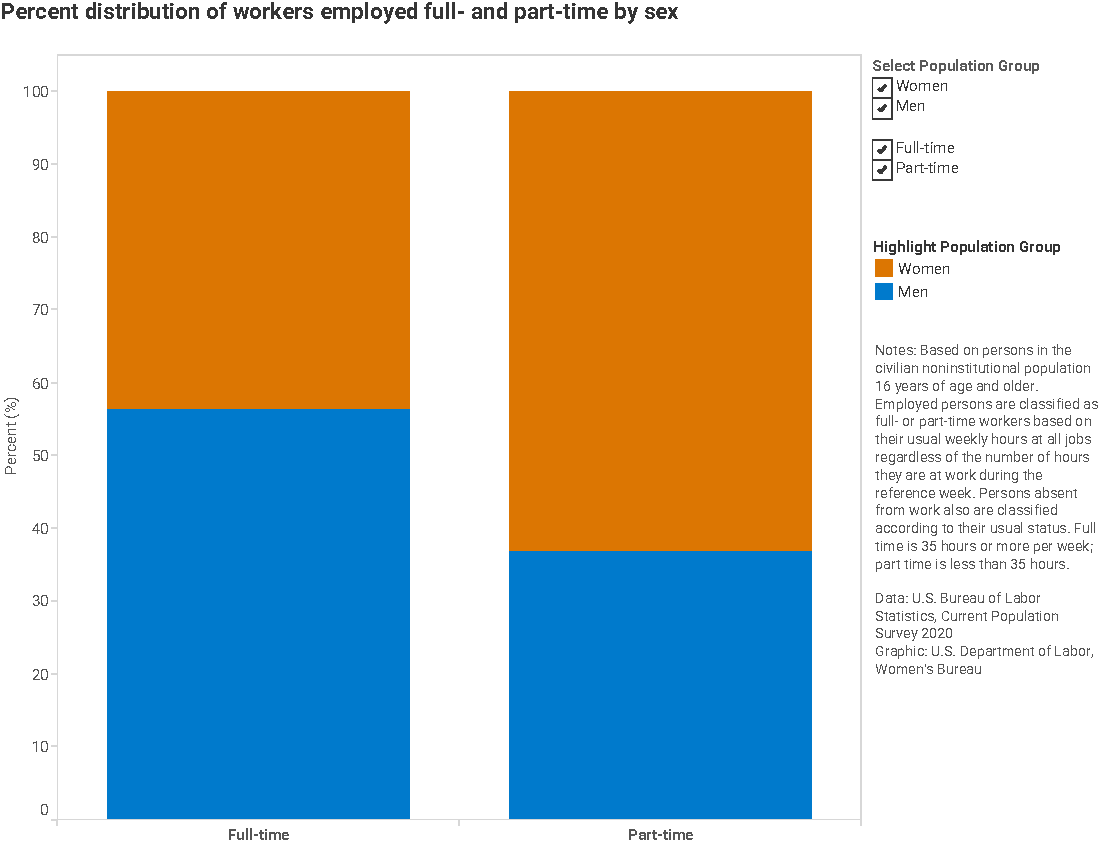
\includegraphics[width=0.475\textwidth]{figures/dol_full-_and_part-time_workers_by_sex.pdf}}
        \end{figure}
    \end{frame}
    
    
    \begin{frame}{Sociological Perspective -- Data \& Statistics}
        \begin{figure}
            \subfloat{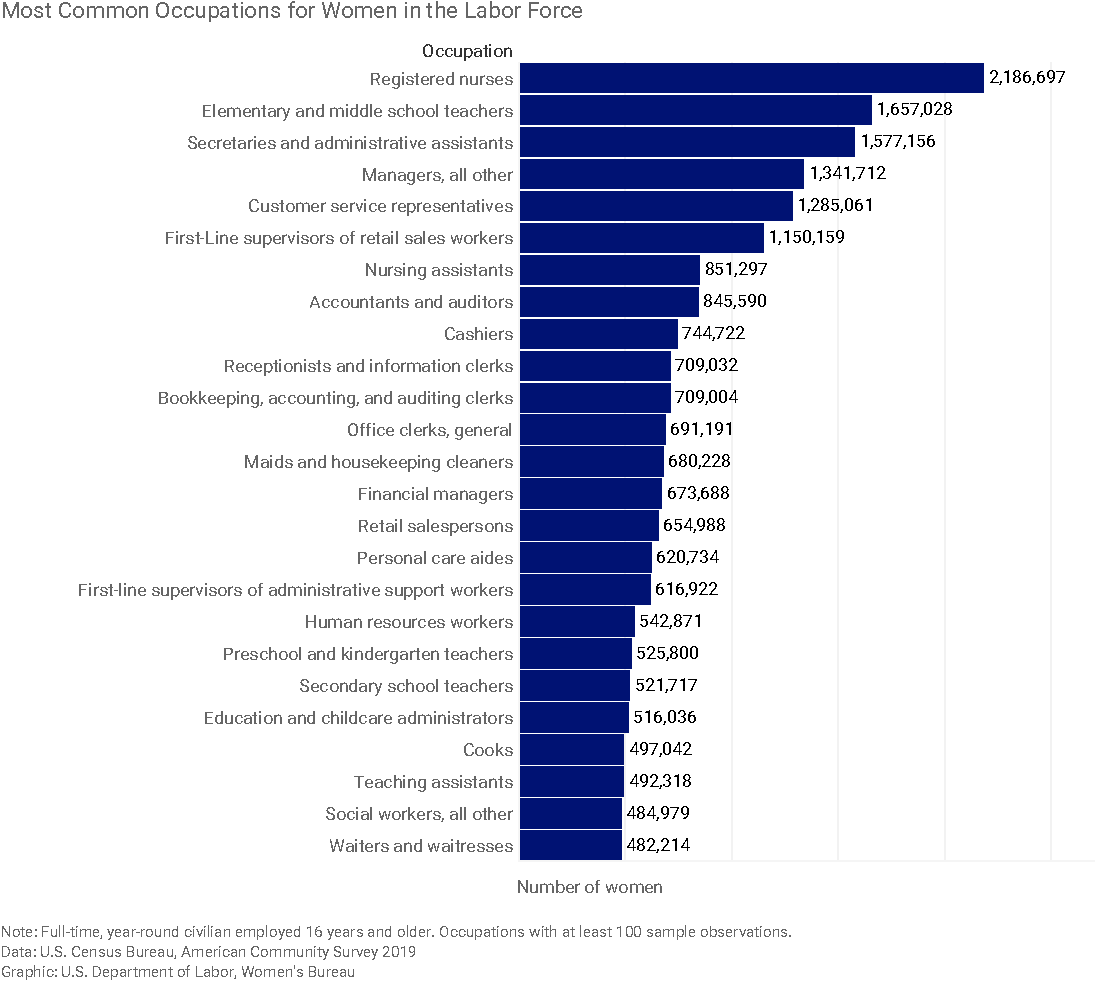
\includegraphics[width=0.475\textwidth]{figures/dol_most_common_occupations_women.pdf}}
            \hfill
            \subfloat{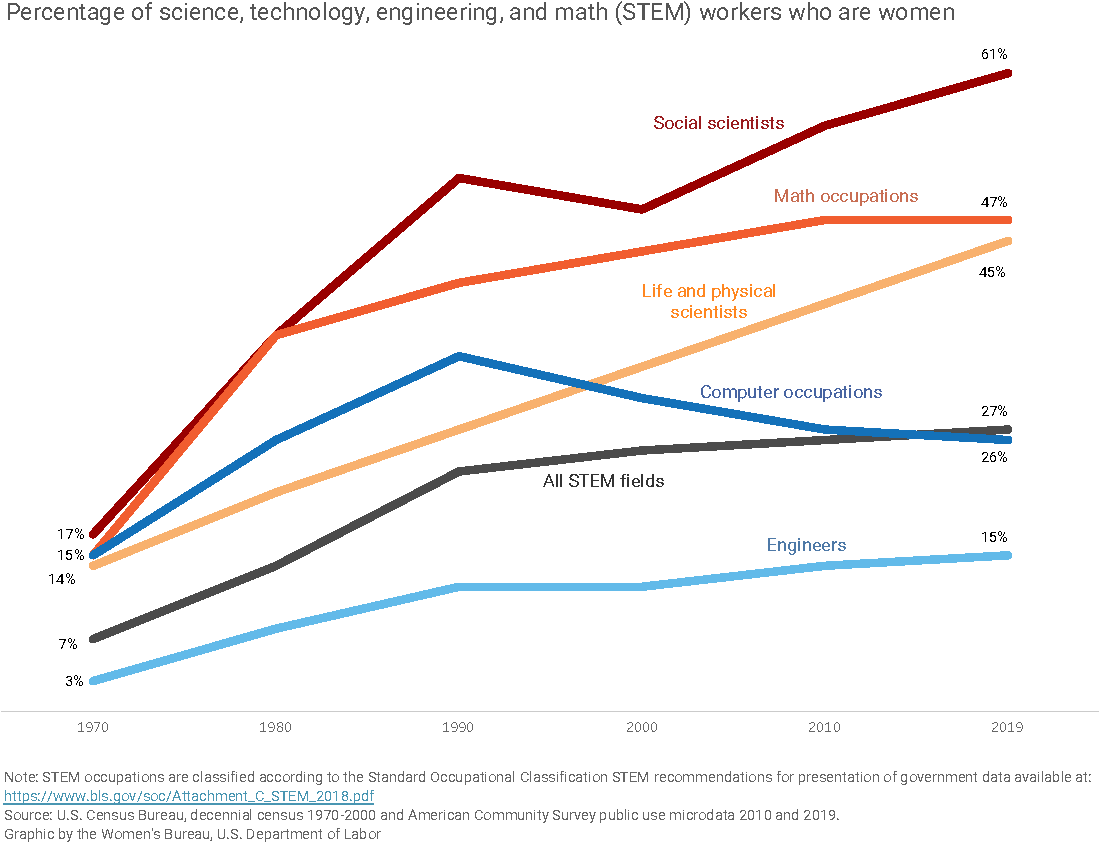
\includegraphics[width=0.475\textwidth]{figures/dol_stem_percent_women.pdf}}
        \end{figure}
    \end{frame}

    
    \section{Section 1}
    % Section page.
    \begin{frame}[plain]{}
        \sectionpage
    \end{frame}
    
    
    \begin{frame}{Slide 1}
        \lipsum[1]
    \end{frame}
    
    
    \subsection{Subsection 1.1}
    \begin{frame}[plain]{}
        \subsectionpage
    \end{frame}
    \begin{frame}
        This frame has an empty title.
        \vfill
        \begin{itemize}
            \item item 1
            \begin{itemize}
                \item item 1.1
                \item item 1.2
            \end{itemize}
            \item item 2
            \item item 3
        \end{itemize}
    \end{frame}
    
    
    \subsection{Subsection 1.2}
    % Slide without numbering.
    \begin{frame}[nonumber]{Slide 1.2 without numbering}
        \lipsum[2]
    \end{frame}
    
    
    \section[Short]{Section 2}
    \begin{frame}{Slide 2}
        \begin{block}{Block}
            Text.
        \end{block}
        \pause
        \begin{alertblock}{Alert block}
            Alert \alert{text}.
        \end{alertblock}
        \pause
        \begin{exampleblock}{Example block}
            Example \textcolor{greenPolimi}{text}.
        \end{exampleblock}
    \end{frame}
\end{document}
